% chktex-file 3 chktex-file 18 chktex-file 36
\section*{Exercise 3.}

Calculate the following integrals with complex analysis methods

\begin{enumerate}[label=(\alph*)]
    \item $\displaystyle \int_{-\infty}^{\infty} \frac{x^2}{x^{4} + 6x^{2}+13} dx$
    \item $\displaystyle \int_{0}^{\infty} \frac{\sqrt{x}}{x^2 + 1} dx$
    \item $\displaystyle \int_{0}^{\infty} \frac{\sin x}{x} dx$
\end{enumerate}

\subsection*{Solution Item (a)}

The difference of the degrees between the denominator and numerator is 2, so we can use the following method

\[ \int_{-\infty}^{\infty} \frac{x^2}{x^{4} + 6x^{2}+13} dx = 2\pi i \sum_{\im(z_0) > 0} \Res_{z = z_0} \left( \frac{z^2}{z^{4} + 6z^{2}+13} \right) \]

The function $z^{4} + 6z^{2}+13$ has a zero with multiplicity 1 at
\[ a = \sqrt[4]{13} \cos\left( \frac{1}{2}\left( \tan^{-1}\left( \frac{2}{3} \right) - \pi  \right) \right) - i\sqrt[4]{13} \sin\left( \frac{1}{2}\left( \tan^{-1}\left( \frac{2}{3} \right) - \pi  \right) \right) \]
It also has multiplicity 1 zeroes at $-\ol{a},\ol{a}, -a$, but the only ones at the upper half plane are $a$ and $-\ol{a}$.

Then,
\[ \everymath{\displaystyle}
\arraycolsep=1.8pt\def\arraystretch{2.5}
\begin{array}{rcl}
    \Res_a f(z) & = & \lim_{z\to a} (z-a)\frac{z^2}{(z-a)(z+a)(z-\ol{a})(z+\ol{a})}\\
    & = & \frac{a^2}{2a(2i \im (a))(2 \re(a))}\\
    & = & \frac{-ia}{8\im(a)\re(a)}
\end{array} \]
\[ \everymath{\displaystyle}
\arraycolsep=1.8pt\def\arraystretch{2.5}
\begin{array}{rcl}
    \Res_{-\ol{a}} f(z) & = & \lim_{z\to -\ol{a}} (z+\ol{a})\frac{z^2}{(z-a)(z+a)(z-\ol{a})(z+\ol{a})}\\
    & = & \frac{\ol{a}^2}{(-2 \re(a))(-2i \im (a))(-2\ol{a})}\\
    & = & \frac{-i\ol{a}}{8\im(a)\re(a)}
\end{array} \]

Finally,
\[ \everymath{\displaystyle}
\arraycolsep=1.8pt\def\arraystretch{2.5}
\begin{array}{rcl}
    \frac{1}{2\pi i}\int_{-\infty}^{\infty} \frac{x^2}{x^{4} + 6x^{2}+13} dx & = & \Res_a f(z) + \Res_{-\ol{a}} f(z)\\
    & = & \frac{-ia - i\ol{a}}{8\im(a)\re(a)}\\
    & = & \frac{i(-2 \re(a))}{8\im(a)\re(a)}\\
    & = & \frac{-i}{4 \im(a)}\\
    & = & \frac{i}{4 \sqrt[4]{13} \sin\left( \frac{1}{2}\left( \tan^{-1}\left( \frac{2}{3} \right) - \pi  \right) \right)}\\
\end{array} \]
So it follows that 
\[ \int_{-\infty}^{\infty} \frac{x^2}{x^{4} + 6x^{2}+13} dx = \frac{-2\pi}{4 \sqrt[4]{13} \sin\left( \frac{1}{2}\left( \tan^{-1}\left( \frac{2}{3} \right) - \pi  \right) \right)} \approx 0.8643 \]
\begin{figure}[H]
    \centering
    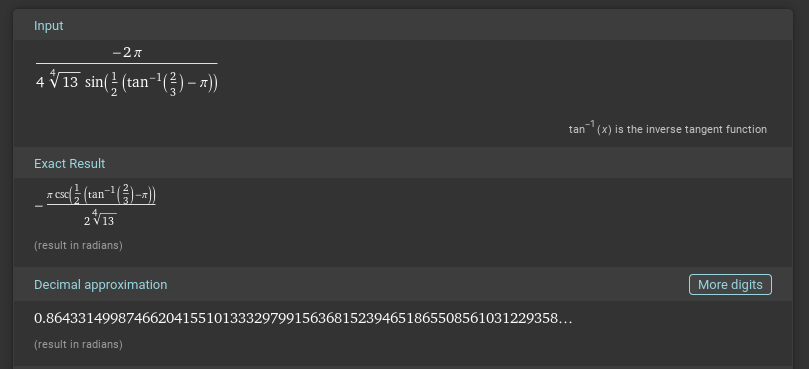
\includegraphics[width=0.85\textwidth]{../pictures/image1.png}
\end{figure}
and this coincides with the real result
\begin{figure}[H]
    \centering
    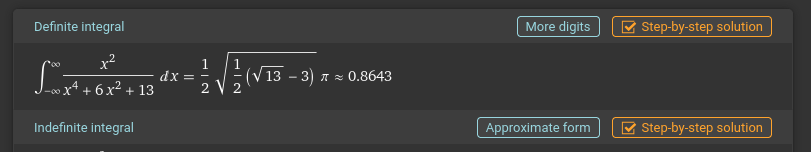
\includegraphics[width=0.85\textwidth]{../pictures/image2.png}
\end{figure}

\subsection*{Solution Item (b)}
This integral has the form $\int_0^{\infty} x^\alpha R(x)$ where $0< \alpha = 1/2 < 1$ and $R(x) = O(x^{-2})$ without any poles at the origin. Therefore, by using the substitution $ x = t^2$, $dx = 2t dt$, we obtain
\[ \everymath{\displaystyle}
\arraycolsep=1.8pt\def\arraystretch{2.5}
\begin{array}{rcl}
    \int_{0}^{\infty} x^{\alpha} R(x) dx & = & 2 \int_{0}^{\infty} t^{2\alpha +1 }R(t^2) dt\\
    & = & \int_{-\infty}^{\infty} t^{2\alpha +1 }R(t^2)  dt\\
    & = & \int_{-\infty}^{\infty} \frac{t^2}{t^4+1} dt
\end{array} \]
It follows that since the difference between the degrees of the denominator and numerator is two,
\[ \int_{0}^{\infty} \frac{\sqrt{x}}{x^2+1} dx = \sum_{\im(z_0) > 0} \Res_{z = z_0} \left(  \frac{z^2}{z^4+1} \right)\]
The polynomial $z^4 + 1$ has a root of multiplicity 1 at
\[ a = \frac{1+i}{\sqrt{2}} \]
and also has roots at $-a,\ol{a},-\ol{a}$, from which only $a$ and $-\ol{a}$ are in the upper half plane. Using the same logic as the previous item (because it's the exact same case only changing the value of $a$),
\[ \everymath{\displaystyle}
\arraycolsep=1.8pt\def\arraystretch{2.5}
\begin{array}{rcl}
    \Res_a f(z) & = & \lim_{z\to a} (z-a)\frac{z^2}{(z-a)(z+a)(z-\ol{a})(z+\ol{a})}\\
    & = & \frac{-ia}{8\im(a)\re(a)}
\end{array} \]
\[ \everymath{\displaystyle}
\arraycolsep=1.8pt\def\arraystretch{2.5}
\begin{array}{rcl}
    \Res_{-\ol{a}} f(z) & = & \lim_{z\to -\ol{a}} (z+\ol{a})\frac{z^2}{(z-a)(z+a)(z-\ol{a})(z+\ol{a})}\\
    & = & \frac{-i\ol{a}}{8\im(a)\re(a)}
\end{array} \]
So finally,
\[ \everymath{\displaystyle}
\arraycolsep=1.8pt\def\arraystretch{2.5}
\begin{array}{rcl}
    \frac{1}{2\pi i}\int_{-\infty}^{\infty} \frac{t^2}{t^{4} + 1} dt & = & \Res_a f(z) + \Res_{-\ol{a}} f(z)\\
    & = & \frac{-ia - i\ol{a}}{8\im(a)\re(a)}\\
    & = & \frac{i(-2 \re(a))}{8\im(a)\re(a)}\\
    & = & \frac{-i}{4 \im(a)}\\
    & = & \frac{-i}{4\sqrt{2}},
\end{array} \]
and thus,
\[ \int_{0}^{\infty} \frac{\sqrt{x}}{x^2+1} dx = 2 \int_{-\infty}^{\infty} \frac{t^2}{t^{4} + 1} dt = \frac{\pi}{\sqrt{2}} ,\]
which coincides with the real result
\begin{figure}[H]
    \centering
    
\includegraphics[width=0.85\textwidth]{../pictures/image3.png}
\end{figure}

\subsection*{Solution Item (c)}

We have that
\[ \everymath{\displaystyle}
\arraycolsep=1.8pt\def\arraystretch{2.5}
\begin{array}{rcl}
    \int_{0}^{\infty} \frac{\sin x}{x} dx & = & \int_{0}^{\infty} \frac{e^{ix}- e^{-ix}}{2i x} dx\\
    & = & \int_{0}^{\infty} \frac{e^{ix}}{2i x} dx - \int_{0}^{\infty} \frac{e^{-ix}}{2i x} dx\\
    & = & \int_{0}^{\infty} \frac{e^{ix}}{2i x} dx + \int_{-\infty}^{0} \frac{e^{ix}}{2i x} dx\\
    & = & \int_{-\infty}^{\infty} \frac{e^{ix}}{2i x} dx
\end{array} \]
We have a simple pole at $x = 0$ and $R(\infty) = 0$, so we can apply the following formula
\[ \everymath{\displaystyle}
\arraycolsep=1.8pt\def\arraystretch{2.5}
\begin{array}{rcl}
    \int_{-\infty}^{\infty} \frac{e^{ix}}{x} dx & = & \int_{-\infty}^{\infty} R(x) e^{ix} dx\\
    & = & 2\pi i \sum_{\im(z_0) > 0} \Res_{z = z_0}R(z)e^{iz} + \pi i \sum_{\im(z_0) = 0} \Res_{z = z_0}R(z)e^{iz}\\
    & = & \pi i \Res_{z = 0} \frac{e^{iz}}{z} = \pi i.
\end{array} \]
Finally,
\[ \int_{0}^{\infty} \frac{\sin x}{x} dx = \frac{1}{2i}\int_{-\infty}^{\infty} \frac{e^{ix}}{x} dx = \frac{\pi}{2} \]

\begin{figure}[H]
    \centering
    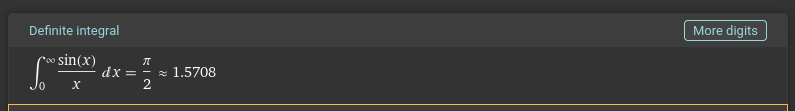
\includegraphics[width=0.85\textwidth]{../pictures/image4.png}
\end{figure}